\documentclass[a4paper,10pt, bibliography=totocnumbered]{scrreprt}

\usepackage[utf8x]{inputenc}
\usepackage[english]{babel}

\usepackage{graphicx}
\usepackage{pdfpages}
%\usepackage{subfig}
%\usepackage{microtype}
\usepackage{tabularx}
%\usepackage{amsmath, textcomp}

% Custom packages
\usepackage[numbers]{natbib}
\usepackage{ragged2e}
\usepackage{longtable}
%\usepackage{tikz}
%\usetikzlibrary{positioning}
%\usepackage{pdflscape}
%\usepackage{rotating}

%----------Begin Hausberger Packages-----------
%\usepackage{csquotes}
%\usepackage{float}
\usepackage{longtable}
\usepackage{listings}
\usepackage{color}

\definecolor{dkgreen}{rgb}{0,0.6,0}
\definecolor{gray}{rgb}{0.5,0.5,0.5}
\definecolor{mauve}{rgb}{0.58,0,0.82}

\lstset{
	frame=tb,
	language=Java,
	aboveskip=3mm,
	belowskip=3mm,
	showstringspaces=false,
	columns=flexible,
	basicstyle={\small\ttfamily},
	morekeywords={UC, context, pre, @pre, post, and, or, not, implies, forall, exists},
	numbers=none,
	numberstyle=\tiny\color{gray},
	keywordstyle=\color{blue},
	commentstyle=\color{dkgreen},
	stringstyle=\color{mauve},
	breaklines=true,
	breakatwhitespace=true,
	tabsize=3
}
%----------End Hausberger Packages-----------

\usepackage{glossaries} 

\usepackage{hyperref}
\hypersetup{
    colorlinks=true,        % false: boxed links; true: colored links
    linkcolor=black,        % color of internal links
%    citecolor=green,        % color of links to bibliography
    citecolor=black,        % color of links to bibliography
    filecolor=magenta,      % color of file links
    urlcolor=blue           % color of external links
}


%% Title Page
\makeatletter
\renewcommand{\maketitle}{\begin{titlepage}
    \vskip 10\p@
    \hbox{
      \vrule depth 0.99\textheight
        \mbox{\hspace{2em}}
      \vtop{
        \vskip 10\p@
        \hspace{4pt}
        \vskip 50\p@
        \begin{flushleft}
          \Large \@author \par
        \end{flushleft}
        \vskip 50\p@
        \begin{flushleft}
          \huge \bfseries \@title \par
        \end{flushleft}
        \begin{flushleft}
          \Large \bfseries \@subtitle \par
        \end{flushleft}
        \vskip 70\p@
        \begin{flushleft}
          \Large \@publishers \par
        \end{flushleft}
        \vskip 50\p@
        \begin{flushleft}
          \Large \@date \par
        \end{flushleft}
        }}
  \end{titlepage}
}
\makeatother

\author{Author 1, Author n}
\title{Title }
\subtitle{Technical Report}
\publishers{\textbf{Advisor University of Heidelberg}\\ Prof. Dr. Barbara Paech, Astrid Rohmann}
\date{mm dd, year}



% Deutsche Absaetze:
\parindent 0pt
\parskip 12pt

\textwidth145mm
\setlength{\oddsidemargin}{0.7cm}
\setlength{\topmargin}{-0.5cm}
\setlength{\textheight}{22.5cm}

\begin{document}
\maketitle

\begin{abstract}
\section*{Abstract}

Testing is an essential and time-consuming part of any software development.
This work is a collaboration that highlights various approaches to how systematic tests can be created to make this process more efficient, clearer, easier or more successful.
After the introduction for this purpose eight different methods are dealt with in own subchapters.
Each of these chapters deals with the investigated approach, describes the problem, discusses the literature search on the topic, and then compares the approaches found in each case via a synthesis matrix.
The approaches are put into practice using the example of a movie manager.
Subsequently, the topic described in this subchapter is summarized and a statement regarding the usage for a systematic test generation is made. 

The first topic dealt with is \enquote{systematic generation of acceptance tests that are executable with FitNesse}.
It is about generating automatic tests with the tool FitNesse.
This approach tries to solve the difficulties of communication among the participants.
For this purpose several artifacts like the fit tables are created and used.
After the investigation, it is concluded that the approaches can work well depending on the project size and experience, but unfortunately it is highly dependent on the latter in particular. 

The next chapter discusses that it should be possible to generate test cases in early phases of development.
\enquote{Transition systems} can help to derive test cases from specifications.
The approaches examined here offer industry standard solutions, but the capability of generating robustness tests for fault detection is still a weakness.

The third subchapter deals with \enquote{Testing with a timing component}.
The difficulty of integrating individual software components into an overall project is described as a problem.
The aspect particularly considered here is the temporal component, since in many real-time systems the exact time between two instruction executions can lead to different results.
After an analysis, the conclusion is drawn that this is still a rarely used approach with many non-automated working steps. 

In the next chapter, approaches for model-based systems are examined.
First and foremost, these include \enquote{classification trees}.
The goal is to derive automatic test cases based on the requirements and the input parameters of a model.
In conclusion, classification trees are described as well arranged and close to the requirements, but can potentially produce many test cases.
Moreover, it is difficult to apply these approaches to systems without a simulated model.

The fifth subchapter focuses on \enquote{model based testing} and examines approaches to make testing with models better and describes the differences between system models and test models.
After the analysis the difficulties in using the tools given in literature are worked out.
Nevertheless, it is possible to reduce test time and errors by using them. 

The initial problem for the next chapter with \enquote{Testing functional and nonfunctional requirements in User Requirements Notation} is the risk for wrong test cases during manual test creation.
User requirements notation should fulfill requirements during test creation and thus prevent incorrect or incomplete tests.
At the end, the problem is discussed that this approach is largely unexplored.
Provided that one makes the effort to take additional steps in test case generation, one still achieves a better quality.

In \enquote{Testing Non-Functional Requirements with Risk Analysis} the focus is on risk analysis, because it is precisely here that error-prone components can be discovered.
Suitable approaches are then sought.
Among the findings here are the importance of automated tests and that tests for non-functional requirements should have more priority. 

The last chapter describes the \enquote{Testing Non-Functional Requirements with Aspects} and puts thereby in the comparison with the previous section the focus on the \enquote{aspects}.
This is intended to describe system-wide functionalities in order to be able to deal with concerns at system level.
Also here the missing availability of tools and suitable research are criticized.
However, the approaches considered seem promising and should be further refined.

Thus, this joint work addresses the merits and difficulties of various test case generation techniques.
Common problems identified are the lack of availability of tools or research, but in suitable use cases most approaches help in improving or automating the test cases.
A final conclusion on this is drawn at the end of this work.

\end{abstract}

\tableofcontents

\chapter{Introduction}\label{sec:introduction}

% Reviewfragen
% - Weckt die Einleitung das Interesse der LeserInnen am Thema?
% - Enthält die Einleitung eine detaillierte Problembeschreibung
%   der Herausforderungen in der Softwareentwicklung, die mit systematischer
%   Testerstellung adressiert werden sollen?
% - Enthält die Einleitung die wesentlichen Aussagen aus den Einleitungen der einzelnen Kapitel?

% Die Einleitung (1 Introduction) des Berichts soll das Interesse der LeserInnen
% am Thema wecken und die gemeinsamen Grundlagen beschreiben. Sie enthält eine
% detaillierte Problembeschreibung der Herausforderungen in der Softwareentwicklung,
% die durch systematische Testerstellung adressiert werden sollen. Zudem enthält sie
% die wesentlichen Aussagen aus den Einleitungen der einzelnen Kapitel 
\section{Systematic Software Testing}\label{sec:introduction_software_testing}

With the rise of smart gadgets and the Internet of Things, more and more parts of our daily life involve technology.
And the software required to run our smartphones, computers and other gadgets  becomes more complex as more data can be processed.
As software becomes more complex, bugs and even small configuration mistakes can have immense consequences as recent data breaches have shown\footnote{\enquote{235 Million Instagram, TikTok And YouTube User Profiles Exposed In Massive Data Leak}, \url{https://www.forbes.com/sites/daveywinder/2020/08/19/massive-data-leak235-million-instagram-tiktok-and-youtube-user-profiles-exposed/}, last visited on 2021-02-10}.
Furthermore, not testing software can have legal consequences.
If basic security measures are not implemented and tested, businesses may violate the \enquote{General Data Protection Regulation}\footnote{see \url{https://eur-lex.europa.eu/legal-content/EN/TXT/?uri=CELEX\%3A02016R0679-20160504&qid=1614251901149}, last visited on 2021-02-25}
(GDPR) and may have to pay fines.
This is not a hypothetical risk.
The \enquote{GDPR Enforcement Tracker}\footnote{see \url{https://www.enforcementtracker.com/}, last visited on 2021-02-10} lists instances where businesses had to pay fines due to \enquote{Insufficient technical and organisational measures to ensure information security}.

Therefore, proper testing of software becomes more important than ever.
But what is software testing? According to the \enquote{Guide to the Software Engineering Body of Knowledge} (short: SWEBOK), \enquote{Software testing consists of the dynamic verification that a program provides expected behaviors on a finite set of test cases, suitably selected from the usually infinite execution domain.}~\cite{SWEBOK}
This means that it may not even be possible to test every input against the expected output, for example if the input is an infinite data stream.
But also for functionality with a finite set of input data, testing every possible combination may not be feasible.
Software testing can take more time than developing the program under test. Hence, software testing can be tedious, difficult and expensive.
So the question arises how software can be tested in an effective and efficient way.

We need to write tests in a systematic way.
This paper contains 9~articles, % TODO: Hat einer aufgehört?
each describing another approach to systematic software testing.

In \autoref{sec:topic_2} % Fitnesse
we focus on acceptance tests with FitNesse.
Communicating requirements between customers and developers can be difficult.
Whereas natural language can be too ambiguous, code can be too technical.
By using FitNesse, human-readable Fit-Tables which include test steps are created that can be understood by customers. By writing fixture classes, these Fit-Tables can be used to automatically run tests.

But having tests may not be enough.
Which requirement is covered by which test?
Can we be sure that the implementation matches the specification?
Traceability becomes necessary and is required to not loose overview over the tests cases and covered requirements.
This is where
\autoref{sec:topic_3} % Transition System
comes into play with transition systems which can be used to automatically create test paths through the application by using formal specifications.

% Notes: Often specification and implementation does not match; traceability issues: which requirement is covered by which test? Solution: Transition system;

After that,
\autoref{sec:topic_4} % Timing Component
looks into testing with a timing component, since for real-time systems, timing is crucial.
In real-time systems, the exact time between two instructions or variances in the individual execution time can lead to different system reactions and therefore different results.

% The aspect particularly considered here is the temporal component, since in many real-time systems the exact time between two instruction executions or variances in the individual execution time can lead to different results.

% Notes: some times issue can only be found if components are linked together; test with same input but different execution time can lead to different reactions in a real-time system.

Following this,
\autoref{sec:topic_5} % Classiciation Tree
looks into decreasing the number of test cases by using classification trees.
Because testing all possible parameter cases becomes unmanageable very fast, these classification trees offer a great way to reduce the complexity of such parameter constructs.
Furthermore, these classification trees can be used to generate test cases.

% Notes: Testing all possible cases becomes unmanageable very fast.Classification Trees offer an approach to offer an approach to reduce the complexity of such parameter con-structions  and  to  keep  them  clearly  arranged.  Test cases can be generated from CTs

\autoref{sec:topic_6} %TODO % Formal specification
\textit{is missing}
% Noch nicht online

In \autoref{sec:topic_7} %  System models
we then look into testing with systems models which are compared against test models.
It is looked into model based testing and how traceability can be used to increase the probability of finding errors and improve test quality.

% KEIN autoref, da sonst kleingeschrieben
Chapter~\ref{sec:topic_8} % NFR/FR Use Requiremetn
explains why writing manual tests for functional and non-functional requirements can be  not only tedious but error prone due to Copy\,\&\,Paste of errors in test logic.
The section describes how test cases can be automatically created by using the user requirements notation that is used for modeling, analyzing, and controlling the correctness and completeness of functional and non-functional requirements.

Another aspect of testing non-functional requirements can be by using risk analysis.
This is where \autoref{sec:topic_9} %  Risk Analysis NFR
steps in and briefly shows how non-functional requirements can be tested and how risk analysis can be used to prioritize test cases.
The section also shows how architectural non-functional requirements such as code conventions can be tested.
\autoref{sec:topic_10} % NFR Aspects
expands on this topic by introducing aspects and aspect oriented programming to test and verify non-functional requirements such as software memory limits and memory leaks.

Finally, \autoref{chap:conclusion} concludes this paper and summarizes each article.

% die Beschreibung der gemeinsamen Grundlagen unter Nutzung des Glossars
% und der Wissensgebiete aus SWEBOK. Das Kapitel gibt einen Überblick über
% die Struktur des Berichts.
\section{Common Fundamentals}\label{sec:introduction_common_fundamentals}
All chapters build upon a common set of fundamental definitions regarding software testing and requirements.
They are listed and mapped to the individual topics in the glossary section of this report.
It is highly recommended to refer to the glossary before reading a chapter or when ambiguities arise while reading a chapter.
However, since it is quite extensive and also contains more topic-specific definitions, the most important terms are defined hereafter.

Like a part of the entries in the glossary section, we use the SWEBOK in its third version as a basis.
Although this guide is already quite old (at least the original version from 2004), hence not fully compliant with current research results, its 15 knowledge areas and basic definitions of a body of knowledge are still useful for classifying the approaches presented in this report and establish a common set of technical terms.

% KEIN autoref, da sonst kleingeschrieben
Let us begin with requirements.
The corresponding SWEBOK knowledge area is \enquote{Software Requirements}.
Relevant sub chapters are \enquote{Software Requirements Fundamentals} and \enquote{Requirements Validation}.
The guide defines requirements as \enquote{a property that must be exhibited by something in order to solve some problem in the real world. [\ldots]
An essential property of all software requirements is that they be verifiable as an individual feature as a functional requirement or at the system level as a non-functional requirement.
It may be difficult or costly to verify certain software requirements.} \cite{SWEBOK}
This definition already points out the difficulty of verifying requirements that necessitates the use of systematic testing techniques, as explained in Section 1.1.
Moreover, it distinguishes between functional requirements, representing a feature the software is to provide, and non-functional requirements, specifying the extend of quality.
Requirements need to be formulated clearly, unambiguously and quantitatively in order to implement and verify them correctly \cite{SWEBOK}.

For software testing, there is no uniform definition.
Therefore, the guide refers to multiple definitions from cited references.
In essence, software testing is to assure that specified requirements are met by the implementation or, from a different perspective, find errors indicating that a requirement has not been met.
This testing process is performed at different levels, as the requirements definition already touched upon.
The SWEBOK guide distinguishes between three test levels: unit testing, verifying isolated functionalities (mostly functional requirements), integration testing, verifying the correct interaction of components and system testing, verifying the behavior of the entire system (mostly non-functional requirements).
Correspondingly, these levels are distinguished by the object of the test (single module, multiple modules, entire system), called the target of the test, and the purpose, called objective of the test \cite{SWEBOK}.

The guide presents a wide array of testing techniques.
For this report, it is important to take notice of the definition of model-based testing: \enquote{A model in this context is an abstract (formal) representation of the software under test or of its software requirements [...].
Model-based testing is used to validate requirements, check their consistency, and generate test cases focused on the behavioral aspects of the software.}\cite{SWEBOK}
Some of the approaches presented in this report are model based, at least partially.
However, it is not always clear what the actual model is and some authors use the term incorrectly.

\section{Outline}
\label{sec:intruduction1.3}

Following this introduction in \autoref{sec:introduction}, nine individual reports each present two different but related approaches for systematic testing in Chapters 2\,-\,10.
The reports introduce their superordinate topic in Sections X.1, outline the results and execution of a literature search based on a given article in Sections X.2 and describe the given and selected approach in Sections X.3.1 and X.4.1 as well as illustrating them using a common set of given requirements in Sections X.3.2 and X.4.2.
Finally, the approaches are compared using a common set of synthesis questions in Sections X.5 and evaluated in Sections X.6.
Chapter 11 concludes the report.
The glossary and bibliography can be found in Chapters 12 and 13.\\

In the following, the given requirements (\autoref{fig:mm}) and synthesis questions, used for each individual report, are depicted.

\newpage
\textbf{Synthesis questions:}

\begin{enumerate}
	\item Description of the approach (What does the approach do?)
	\begin{enumerate}
		\item Which artifacts and relations between artifacts are used in this approach? Which artifacts are created in the course of the approach? How are the artifacts characterized?
		\item What is required and/or input for the application of the approach?
		\item What steps does the approach consist of? Which information is used in which step and how? What are the results of the individual steps?
	\end{enumerate}
	\item[] 
	\item Benefits of the approach (Whom does the approach help and how?)
	\begin{enumerate}
		\item Which usage scenarios are supported by the approach?
		\item Which stakeholders are supported by the usage scenarios?
		\item Which knowledge areas from SWEBOK can be assigned to the usage scenarios?
	\end{enumerate}
	\item Tool support for the approach (What tool support is available?)
	\begin{enumerate}
		\item What tool support is provided for the approach?
		\item Which steps of the approach are automated by a tool? Which steps are supported by a tool, but still have to be executed manually? Which steps are not supported by a tool?
	\end{enumerate}
	\item Quality of the approach (How well does the approach work?)
	\begin{enumerate}
		\item How was the approach evaluated?
		\item What are the (main) results of the evaluation?
	\end{enumerate}
\end{enumerate}


\newpage
\newgeometry{margin=1cm}
\begin{landscape}

\begin{figure}
	\centering
	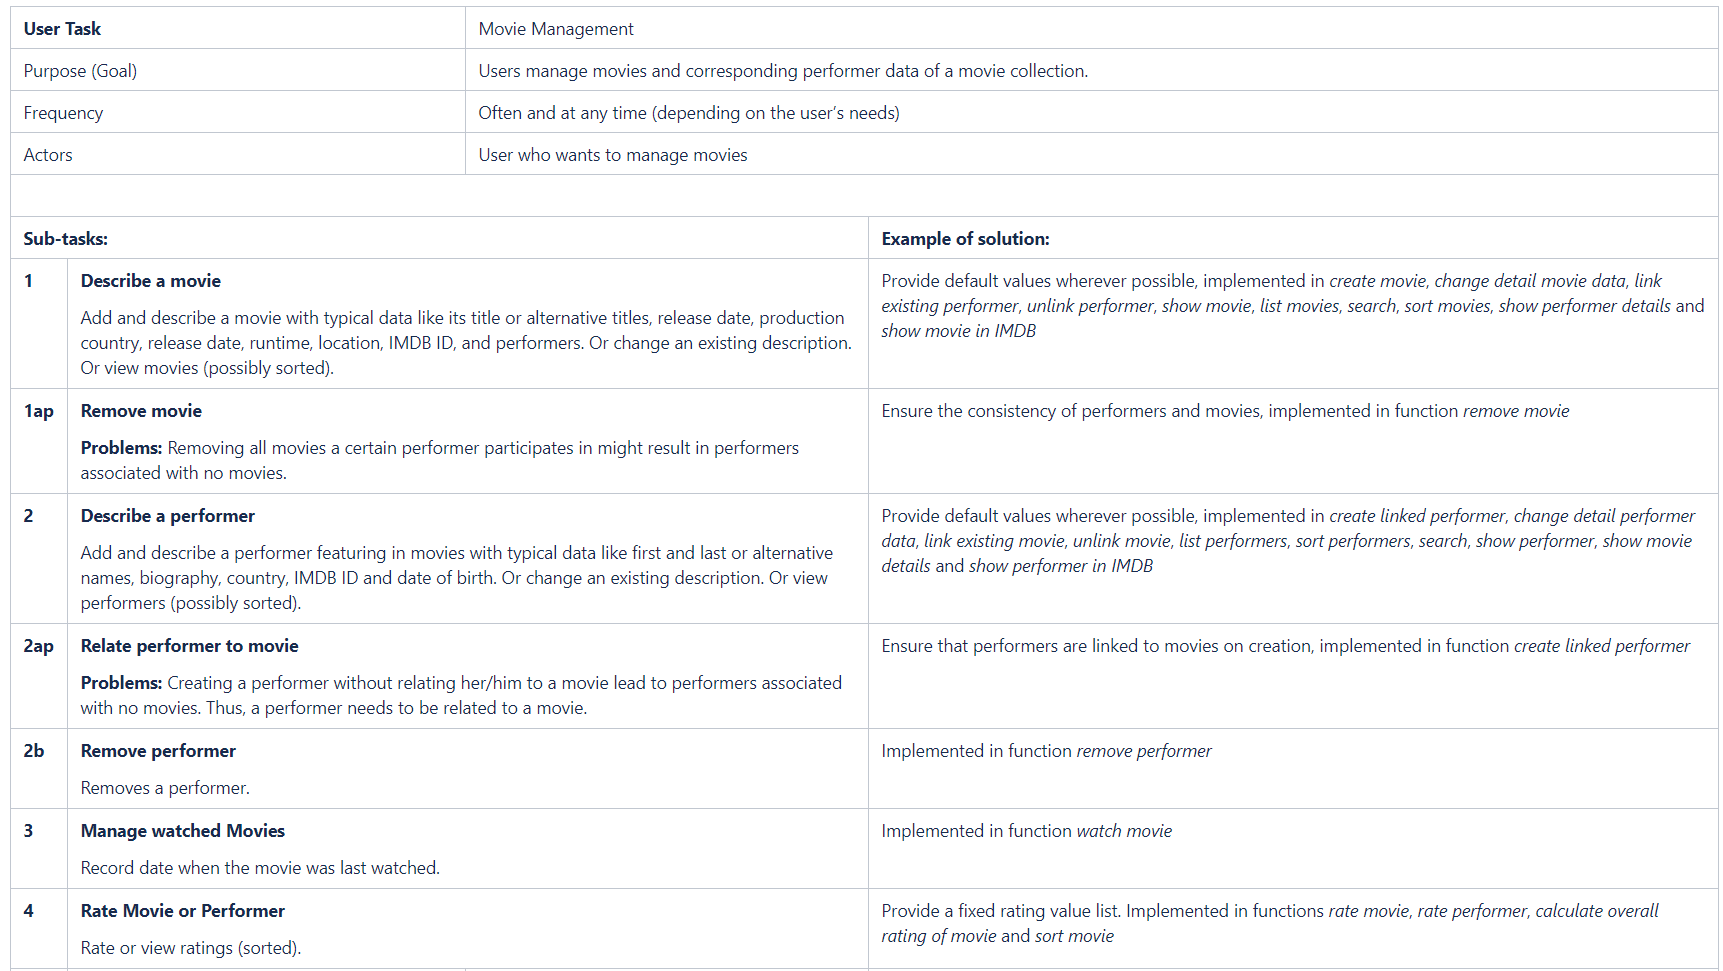
\includegraphics[scale=0.57]{../images/MovieManager.png} 
	\caption{Requirements in User-Task notation for the MovieManager software, an application for managing movie collections.}
	\label{fig:mm}
\end{figure}

\end{landscape}
\restoregeometry



\chapter{Richtiges Zitieren}

1.	Die Seminararbeit ist eine eigenständige wissenschaftliche Arbeit und wird auch nach den Regeln einer wissenschaftlichen Arbeit erstellt (vgl.~\cite{RichtigesZitierenTUDresden}), insbesondere heißt das, dass die Regeln für:
\begin{enumerate}
\item Richtiges Zitieren 
\begin{itemize}
\item Zitierpflicht
\item Zitierregeln
\item Typen von Zitaten
\item Zitierformen
\end{itemize}
\item Literaturangaben 
\item eine gut strukturierte Arbeit 
\end{enumerate}
beachtet und eingehalten werden.




\chapter{Chapter}

Duis porta orci. Integer eu arcu at enim tempus facilisis. Pellentesque dignissim orci sed est. Etiam elementum laoreet mi. Donec nunc sapien, dictum in, tristique sed, aliquam vitae, massa. Morbi magna magna, vestibulum tempor, lobortis non, convallis nec, nibh. In sed nibh. Suspendisse adipiscing dictum pede. Suspendisse non augue. Lorem ipsum dolor sit amet, consectetuer adipiscing elit. Pellentesque lacinia, velit sed commodo convallis, diam dolor consequat ligula, a scelerisque quam neque et purus. Praesent vel augue. Sed lectus leo, dignissim eget, vulputate eu, auctor ut, nulla. Vivamus a quam. Nulla tellus. Pellentesque tempor pulvinar nunc.


\chapter{Testing with a Transition System}

\section{Introduction}

System tests are used to make sure that clients receive exactly the kind of software they previously specified within the order contract submitted to the software vendor. Oftentimes what was specified and what was implemented does not match entirely in the end. The software vendor faces traceability problems to track which requirements could be covered in which tests and therefore which requirements got implemented. How does one make sure that each atomic functional and robustness requirement specified is covered in the requirements' implementation?

To solve this, the process of formal definition of requirements and matching system tests must be brought closer together. Testing should already be possible in early stages of development, to be precise during the specification phase already. To automatically derive test scenarios from means of the specification area \textit{transition systems} are used. They help to generate test paths as possible combinations of fine-grained functional requirements received through the traversal. An equivalent approach can be used to derive robustness tests as well. In this process requirements can furthermore be tested on their consistency, correctness and integration and eventually can be refined further.

For this purpose the two approaches \cite{ClementineNebut2006} and \cite{NajlaRaza2007} were analyzed. While \cite{ClementineNebut2006} was given in advance by the advisors, \cite{NajlaRaza2007} was discovered through an extensive literature search shown in \autoref{literaturesearch}. Both approaches will be explained in the following sections \ref{approachone} and \ref{approachtwo} and applied to the movie management software example. A comparison between the two approaches will be drawn using a synthesis matrix shown in \autoref{comparison}. The main results of testing with transitions systems will be summarized in \autoref{conclusion}. 

Please refer to the glossary in \autoref{glossary} in order to receive a common understanding of the following terms used in the sections below: contract, coverage criterion, interaction overview diagram, object constraint language, operation, test case, test objective, test scenario, transition system, UC-System, UC-SCSystem, use case, use case scenario, XML metadata interchange.

\section{Literature Search} \label{literaturesearch}

The literature research was driven by the central research question: \glqq Which approaches for automatic generation of system tests exist that are using contract enriched use cases or other use case related means of the specification area within a transition system simulation model?\grqq 

The focus during this literature search was on finding a second approach to automatically generate system tests from means of the specification phase by exhaustively simulating a transition system to generate test paths similar to \cite{ClementineNebut2006}. But as \cite{ClementineNebut2006} is restricted on using \textit{contract} enriched \textit{use cases} and \textit{use case scenarios}, the way how \textit{test objectives} are derived was this time freely selectable to receive another new, but similar approach. The pre-search results were promising both on IEEE Xplore and ACM. Only some papers on ACM could not be accessed publicly. The number of results was considered to be sufficient to cover all relevant scientific papers, which is why the research was restricted on these two platforms. Furthermore, two relevance criteria inspired by the central research question were defined:

\begin{itemize}
	\item Does the method described in the article generate system tests automatically from use cases or other use case related means of the specification area?
	\item Are test objectives generated using some kind of simulation model based on use case contracts (pre- and postconditions) or similar transition system approaches?
\end{itemize} 

As system tests can not exclusively be derived from means of the specification area, an article should restrict to generating system tests from use case related means of the specification area. To derive test objectives a transition system should be simulated exhaustively based on contract definitions (pre- and postconditions). 

The search was done using both snowballing and search term techniques. 140 papers were found referencing \cite{ClementineNebut2006} and 46 articles were referenced by \cite{ClementineNebut2006}. The results of the snowballing search can be found in \autoref{snowballing}. The backward snowballing approach was restricted on references stated in the \textit{Related Work} chapter as all other references relate to preceding work that serve as basic knowledge to realize the transition system approach in \cite{ClementineNebut2006}. Additionally, most of the references were quite old since the original paper was published in 2006. Therefore not all papers could be found on IEEE Xplore or ACM. Why specific papers were considered not suitable or only partly suitable is documented in \cite{FelixHausberger2020}.

\begin{table}[h] 
	\centering
	\begin{small}
		\caption{Results of snowballing techniques}
		\label{snowballing}
		\setlength{\tabcolsep}{1em}
		\begin{tabular}{l|c|c|c}
			\hline
			& \textbf{Yes} & \textbf{Possibly} & \textbf{No} \\
			\hline
			\hline	
			Forward snowballing & 5 & 9 & 63 \\
			\hline
			Backward snowballing & 2 & 1 & 2 \\
			\hline
		\end{tabular}
	\end{small}
\end{table}

Seach-term based search was done using the following key terms: system tests, automatic generation, transition system, simulation model, use cases, contracts. Only papers published between 2006 and 2020 having the search term "test" and "use case" in their publication title were evaluated. 

\begin{small}
	\centering
	\begin{longtable}[h]{c|c|p{0.2\textwidth}|p{0.2\textwidth}|c}
		\caption{Results of search-term based technique}\label{search-term}\setlength{\tabcolsep}{1em}\\    %%%%<===
		\hline
		\textbf{Source} & \textbf{Date} & \textbf{Search restrictions} & \textbf{Search query} & \textbf{\#Results} \\
		\hline
		\hline	
		IEEE Xplore & 2020-11-21 & "system tests" in document title; "automatic generation" in document title; "transition system" in full text \& metadata; "simulation model" in full text \& metadata; "use cases" in document title; "contracts" in full text \& metadata; & "system tests" AND "automatic generation" AND "transition system" AND "simulation model" AND "use cases" AND contracts & 0 \\
		\hline
		IEEE Xplore & 2020-11-21 & "system tests" in document title; "automatic generation" in abstract; "transition system" in full text \& metadata; "use cases" in document title; "contracts" in full text \& metadata; & "system tests" AND "automatic generation" AND "transition system" AND "use cases" AND contracts & 0 \\
		\hline
		IEEE Xplore & 2020-11-21 & "test" in document title; "transition system" in full text \& metadata; "use cases" in document title & "system tests" AND "transition system" AND "use cases" & 82 \\
		\hline
		\hline
		ACM & 2020-11-21 & "system tests" in title; "automatic generation" in title; "transition system" in full text; "simulation model" in full text; "use cases" in title; "contracts" in full text; & "system tests" AND "automatic generation" AND "transition system" AND "simulation model" AND "use cases" AND contracts & 0 \\
		\hline
		ACM & 2020-11-21 & "system tests" in title; "automatic generation" in abstract; "transition system" in full text; "use cases" in title; "contracts" in full text; & "system tests" AND "automatic generation" AND "transition system" AND "use cases" AND contracts & 0 \\
		\hline
		ACM & 2020-11-21 & "system tests" in title; "transition system" in full text; "use cases" in title & "system tests" AND "transition system" AND "use cases" & 0 \\
		\hline
		ACM & 2020-11-21 & "test" in title; "use case" in title & "system tests" AND "use cases" & 8 \\
		\hline
	\end{longtable}
\end{small}

From the resulting papers, only one was considered suitable as a potential second paper. After the search for potential articles to be evaluated was finished, a choice between eight remaining papers from the initial search had to be made:

\begin{itemize}
	\item System Testing using UML Models \cite{MonalisaSarma2007},
	\item An Automatic Tool for Generating Test Cases from the System's Requirements \cite{RosziatiIbrahim2007},
	\item Automated Test Case Generation from Use Case: A Model Based Approach \cite{LizheChen2010},
	\item Requirements Document Based Test Scenario Generation for Web Application Scenario Testing \cite{XiaojingZhang2015},
	\item An Approach to Modeling and Testing Web Applications Based on Use Cases \cite{LipingLi2008},
	\item Test cases generation from UML state diagrams \cite{YGKim1999},
	\item Requirements by Contracts allow Automated System Testing \cite{ClementineNebut2003},
	\item An Automated Approach to System Testing Based on Scenarios and Operations Contracts \cite{NajlaRaza2007}.
\end{itemize}

The decision criteria are based on the different search terms mentioned above and the already defined criteria. Additionally, focus of the selected paper should lie on creating system tests for any generic application area, not just UI related parts of an application.

The paper \textit{An Automatic Tool for Generating Test Cases from the System's Requirements} was not chosen as it does not focus on testing the consistency of use case combinations with contracts to build test objectives as in the original paper. Furthermore, it is not as in-depth as the original paper. Contract enriched use cases could neither be found in \textit{System Testing using UML Models}.

\textit{Automated Test Case Generation from Use Case: A Model Based Approach} really embodies the principle of state base modeling based on use cases with its \textit{interaction finite automaton} (IFA), but doesn't introduce a formal language to define use cases and its contracts.

\textit{Requirements Document Based Test Scenario Generation for Web Application Scenario Testing} as well as \textit{An Approach to Modeling and Testing Web Applications Based on Use Cases} are specifically optimized for web application \textit{test scenarios} and therefore not as general and universally applicable as the original paper.

\textit{Test cases generation from UML state diagrams} and \textit{Requirements by Contracts allow Automated System Testing} could unfortunately not be accessed in full length in IEEE Xplore.

The chosen article to further evaluate is \textit{An Automated Approach to System Testing based on Scenarios and Operations Contracts}, as it introduces a second way to create system tests from use case scenarios as UML 2.0 models by enriching it with contracts and by transforming the formalized scenarios to a transition system to derive test objectives. It uses a more graphical approach to define use cases instead of using a formalized language to do so and goes deeper down into use-case level instead of system-level test generation. A more in-depth comparison between the two papers can be found in \autoref{comparison}.

\section{Automatic Test Generation: A Use Case Driven Approach} \label{approachone}

\subsection{Description}

\begin{figure}[h]
	\centering
	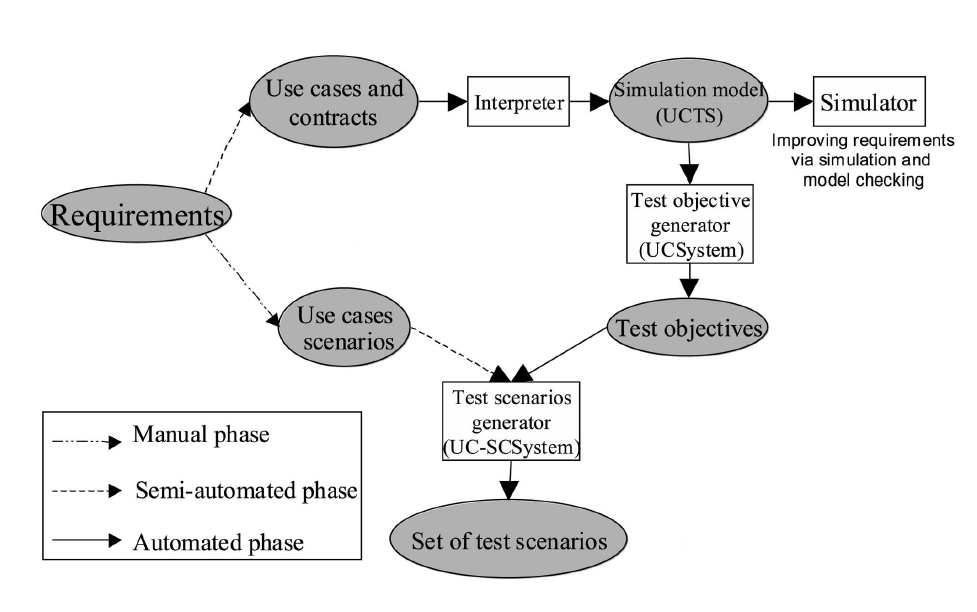
\includegraphics[width=0.75\textwidth]{./images/transitionsystemflow.png}
	\caption{Flow of generating test scenarios \cite{ClementineNebut2006}}
	\label{tsf}
\end{figure}

The approach consists of two phases (see \autoref{tsf}). In the first phase, UML use cases get enhanced with contracts (pre- and postconditions). Use cases can be seen as the systems' main functions whereas contracts are used to infer the correct partial ordering of functionalities that the system should offer. They express the ordering constraints between the use cases during the simulation process to build the transition system. The contracts are made executable by writing them in the form of requirement-level first-order logical expressions. They consist of predicates with logical operators, quantifiers, and implications and are used to describe facts in the system like actor state, main concept state, roles, and more. Each predicate can either evaluate to true or false, but never to undefined. A dedicated editor tool helps to manage the predicates and guides the design of contracts to maintain a nonredundant, minimal set of contracts and predicates. Contracts therefore specify the system properties to make a use case applicable (preconditions) and define the system properties (predicates) acquired after their application (deterministic postconditions). Parameters to use cases can either be system actors or main concepts of the use case, which are represented as normal instantiated objects of classes during the test generation process. 

Through exhaustive simulation by the prototype/interpreter-tool \textit{UC-System} a \textit{use case transition system} (UCTS) is built, which serves as a model for all valid sequences of use cases. Therefore first an initial state and enumerations of different business entities that later serve as parameters to use cases are declared. Then all use cases get instantiated by replacing the set of formal parameters with all the possible combinations of their possible actual values (i.e. actors and main concepts). To apply an instantiated use case the simulation state and the precondition of an instantiated use case must match. The simulation state is then updated according to the postcondition of the contract. The initial state defines which predicates are true from the very beginning, the current simulation state covers all instantiated predicates which are evaluated to true. Now all possible paths are traversed exhaustively until a final UCTS was generated. During this step, the requirement engineer has also the chance to check and possibly correct the requirements before the tests are generated. Inconsistencies between predicates and contracts can be identified as well as underspecification or errors in the requirements. Invariants can also be checked. The number of states in the transition system can be calculated with

\begin{equation}
	maxsize_{UCTS} = 2^{n_{ip}}
\end{equation}

where

\begin{equation}
	n_{ip} = p \cdot max_{instances}^{max_{param}}.
\end{equation}

$n_{ip}$ describes the amount of instantiated predicates, $p$ the number of predicates, $max_{instances}$ the maximum amount of instances, and $max_{param}$ the maximum amount of parameters per predicate p. In practice, many of the potential states are not reachable and only a small number of instances are necessary for achieving a proper statement coverage. 

Now relevant test objectives get extracted from the UCTS by applying predefined \textit{coverage criteria}. 

The \textit{All Edges} (AE) criterion makes sure that all state transitions are covered, whereas the \textit{All Vertices} (AV) criterion guarantees that all states (predicates) are reached within the set of test objectives.  The \textit{All Instantiated Use Cases} (AIUC) criterion is helpful in case a state transition can be done by multiple use cases or a use case leads to no state change. A combination od AV and AIUC is the \textit{All vertices and All Instantiated Use Cases} (AV-AIUC) criterion. The most strict criterion is probably the \textit{All Precondition Terms} (APT) criterion, which makes sure that all possible ways to apply each use case are exercised. Now, these criteria are mainly introduced to generate functional tests. The \textit{Robustness} criterion on the other hand explicitly exercises a use case in as many different ways as to make its precondition false. Therefore valid test paths are generated, which lead to an invalid application of a use case to generate robustness tests from. All algorithms are based on breadth-first search in the UCTS to obtain small test-objectives that are human-understandable and meaningful. 

Subsequently, in the second phase, test scenarios get generated by replacing each use case in a test objective with the according use case scenario that is compatible in terms of static contract matching. This is done by the prototype-tool \textit{UC-SCSystem}. The use case scenarios were also attached with contracts beforehand. This time the contracts contain more detailed pre- and postconditions. There are contracts that rely on the rest of the model, they are written in \textit{Object Constraint Language} (OCL), and there are contracts that rely on the predicates of the use cases. Now the exchange of messages involved between the environment and the system is also specified. Note that all use case scenarios are system-level scenarios. Eventually, additional parameters and messages need to be passed manually before executable \textit{test cases} can be generated. The process results in executable test scenarios that get evaluated using the statement coverage metric.

One possible challenge of the approach is that the simulation model has to be compact enough to avoid combinatorial explosion of the internal states. Therefore the two-phase approach was chosen and parameters to instantiate use cases during the simulation can often be restricted to only the main system concepts and actors. Furthermore, the above-mentioned test objective generation criteria were identified through experimental comparisons and help to keep the number of test objectives in a reasonable scope. 

The generated test scenarios can either lead to a pass verdict, a fail verdict (in case a postcondition is violated), or an inconclusive verdict. The latter is invoked if a precondition is evaluated to false and the test scenario was not executed entirely. This could be because of underspecification or because of inappropriate test data. To solve this either a new initial state (test data) has to be defined or additional test cases that execute the remaining use case scenarios need to be provided. 

To evaluate the approach the original authors used three software products: An Automated Teller Machine (ATM) with 850 lines of code, an FTP server with 500 lines of code, and a virtual meeting (VM) server with 2.500 lines of code. Statistics on the amount of generated test cases can be found in \autoref{testcases}.

\begin{table}[h] 
	\centering
	\begin{small}
		\caption{Statictics of the generated test cases}
		\label{testcases}
		\setlength{\tabcolsep}{1em}
		\begin{tabular}{l|c|c|c}
			\hline
			& \textbf{ATM} & \textbf{FTP} & \textbf{VM} \\
			\hline
			\hline	
			\# use cases & 5 & 14 & 14 \\
			\hline
			\# nominal UC-scenarios & 5 & 14 & 14 \\
			\hline
			\# exceptional UC-scenarios & 17 & 14 & 14 \\
			\hline
			\# generated functional test cases & 6 & 14 & 15 \\
			\hline
			\# generated robustness test cases & 17 & 33 & 65 \\
			\hline
		\end{tabular}
	\end{small}
\end{table}

Taken the example of the VM server, most coverage criteria reached up to 70\% code coverage, when including robustness test cases even up to 80\%. For more detailed information see \autoref{codecoverage}.

\begin{table}[h] 
	\centering
	\begin{small}
		\caption{Statement coverage reached by the generated test cases}
		\label{codecoverage}
		\setlength{\tabcolsep}{1em}
		\begin{tabular}{l|c|c|c}
			\hline
			& \textbf{ATM} & \textbf{FTP} & \textbf{VM} \\
			\hline
			\hline	
			\% of functional code covered & 100\% & 90.7\% & 100\% \\
			\hline
			\% of robustness wrt. the spec covered & 42.31\% & 38.6\% & 52\% \\
			\hline
			\% of code covered (total) & 94.76\% & 72.5\% & 80\% \\
			\hline
		\end{tabular}
	\end{small}
\end{table}

All coverage criteria are almost equal in their achieved code coverage, with the exception of the AV criterion. Here the code coverage is low as not all use cases can be covered, especially those use cases that do not change the system state are missing. The ratio between the covered statements and the amount of generated test cases gives information about the efficiency of the generated test scenarios. Here the AIUC and APT criteria scored best. The APT criterion manages to reach 100\% functional code coverage with only 15 test cases. The efficiency of the robustness criterion on the other hand scored quite low, 65 test cases could only cover up to 50\% of the equivalent robustness code. Therefore the approach works well for functional code, but not so well for robustness code. This is because only violations of the use case attached preconditions are taken into account, inappropriate test data, or violating the more detailed preconditions of use case scenarios are not included in the test generation process. 

One possible extension of the approach was also considered. Activity diagrams could be chosen to model the use case dependencies in a more graphical approach, which is then shown in the upcoming approach two. 

\subsection{Application}

In the first step, the test objectives have to be derived. Therefore we define the use cases and their contracts (\autoref{contracts1}) as requirement-level first-order logical expressions. The contracts are used to infer the correct partial ordering of functionalities that the system should offer. Only the use cases that really impact the state of the transition system were specified for this example. The notation used is equal to the one proposed in the paper. \textit{UC} introduces the identifier and parameters of a use case, \textit{pre} marks the beginning of the precondition logical expression and \textit{post} the beginning of the postcondition logical expression. 

\begin{lstlisting}[caption={Contracts attached to use cases},label={contracts1}]
	
	UC createMovie(m: movie)
	post createdMovie(m)
	
	UC createLinkedPerformer(p: performer, m: movie)
	pre createdMovie(m)
	post createdPerformer(p) and createdLink(p,m)
	
	UC rateMovie(m: movie)
	pre createdMovie(m)
	post calculatedOverallRating(m)
	
	UC ratePerformer(p: performer)
	pre createdPerformer(p)
	post forall(m: movie){ createdLink(p,m)@pre implies calculatedOverallRating(m) }
	
	UC linkExistingMovie(m: movie, p: performer)
	pre createdMovie(m) and createdPerformer(p)
	post not createdLink(p,m)@pre implies (createdLink(p,m) and calculatedOverallRating(m))
	
	UC linkExistingPerformer(m: movie, p: performer)
	pre createdMovie(m) and createdPerformer(p)
	post not createdLink(p,m)@pre implies (createdLink(p,m) and calculatedOverallRating(m))
	
	UC unlinkMovie(m: movie, p: performer)
	pre createdMovie(m) and createdPerformer(p) and createdLink(p,m)
	post calculatedOverallRating(m) and not createdLink(p,m) and not exists(m2: movie){ createdLink(p,m2) }@pre implies not createdPerformer(p)
	
	UC unlinkPerformer(m: movie, p: performer)
	pre createdMovie(m) and createdPerformer(p) and createdLink(p,m)
	post calculatedOverallRating(m) and not createdLink(p,m) and not exists(m2: movie){ createdLink(p,m2) }@pre implies not createdPerformer(p)
	
	UC removeMovie(m: movie)
	pre createdMovie(m)
	post not createdMovie(m) and forall(p: performer){ not createdLink(p,m) } and not exist(m2: movie){ createdLink(p,m2) }@pre implies not createdPerformer(p)
	
	UC removePerformer(p: performer)
	pre createdPerformer(p)
	post not createdPerformer(p) and forall(m: movie){ not createdLink(p,m) and calculatedOverallRating(m) }
\end{lstlisting}

After that, the UC-System prototype/interpreter tool should build the UCTS (\autoref{ucts}) through exhaustive simulation. The pool of parameters was restricted to one movie and performer to avoid a combinatorial explosion for this example. To build instantiated use cases the set of formal parameters are replaced with all the possible combinations of their actual values. In our case, we use the most simple approach by just having one possible combination. Furthermore, the predicate calculatedOverallRating is no longer considered. Note that only predicates that evaluate to true are listed in the states as in the original paper. 

\begin{figure}[h]
	\centering
	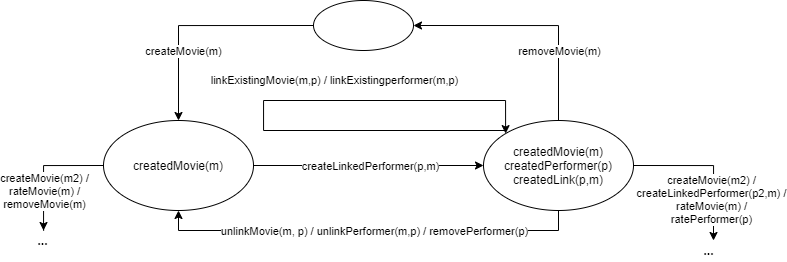
\includegraphics[width=0.85\textwidth]{./images/ucts.png}
	\caption{The use case transition system}
	\label{ucts}
\end{figure}

After applying an instantiated use case in the transition system (in case the precondition of the contract was fulfilled) the simulation state is updated according to the contracts' postcondition. 

Depending on the selected coverage criterion, we receive different test objectives as correct sequences of use cases. The robustness criterion was not considered in this example, but its application is coherent to the functional coverage criteria. How many test objectives are derived depends on the internal implementation of UC-System and cannot be predicted for this example. Let's assume that one test objective is the test path createMovie(m) \mbox{-\textgreater} createLinkedPerformer(p,m) \mbox{-\textgreater} removeMovie(m). Then the use case scenarios from \autoref{ucs} are used to replace the use cases in the test objectives. It helps to specify the exchange of messages involved between the environment and the system.

\begin{figure}[h]
	\centering
	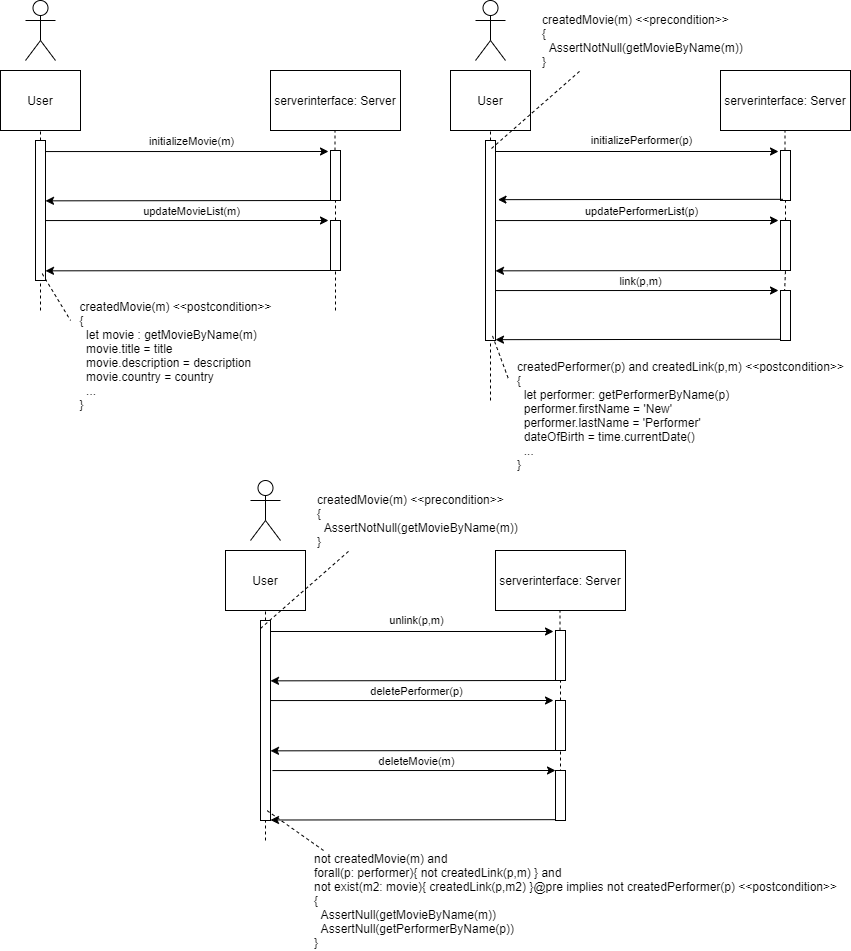
\includegraphics[width=1.0\textwidth]{./images/ucs.png}
	\caption{The use case scenarios}
	\label{ucs}
\end{figure}

Note that the use case scenarios may still be incomplete for the execution. They contain the main messages exchanged between the tester and the SUT and say how the system has to be simulated to perform a use case and how to react to the simulation. To know how the system has to be simulated, the use case scenarios contain more detailed contracts written in OCL besides the contracts written as logical expressions that were provided by the use cases. 

The prototype-tool UC-SCSystem uses the shown implementation in the use case scenarios to derive executable test scenarios as JUnit tests.

\section{An Automated Approach to System Testing based on Scenarios and Operations Contracts} \label{approachtwo}

\subsection{Description}

Based on the suggested improvements in the first paper, the second paper uses a more graphical approach using \textit{interaction overview diagrams} (IOD), a special form of activity diagram used to show control flow, to derive test paths. It helps to start testing in the early stages of development. Each node in the IOD represents either an interaction diagram (sequence diagrams) or interaction occurrences that show an \textit{operation} invocation. Every IOD corresponds to one use case. The IODs get enhanced with contracts written in the \textit{object constraint language} (OCL) and they get transformed into a contracts transition system (CTS) which models all scenarios of the IOD. Here the states are represented by the contracts and the transitions by the operations (interaction diagrams or interaction occurrences) in the IOD. The CTS is built by a tool using the \textit{XML metadata interchange} (XMI) file for the IOD and the operation contracts in OCL as inputs. A state is created against each precondition and each postcondition of the operations. Logical if-then-else conditions are resolved by combining their testing condition with the result, therefore two different sub-states are created. The surrounding postcondition is then a composition of the two sub-states. Additional transitions are added for all conditional flows leading to alternative scenarios and their guard conditions are attached to them. Additional CTS flows help to further refine the requirements by spotting potential unwanted behavior or underspecification. The CTS is often visualized in a matrix. 

Through traversing the CTS test paths get derived. Therefore different coverage criteria are defined. The simplest coverage criterion is the \textit{state coverage} criterion, which generates test paths until all states of the CTS are covered. The criterion is already covered by the wider \textit{transition coverage} criterion, which makes sure that all transitions are traversed before stopping the test path generation. The most expensive criterion is the \textit{transition pair coverage} criterion, each possible transition pair needs to be covered in the test path generation process. It was detected, that the transition coverage criterion delivers a reasonable amount of test paths, but is not suitable for fault detection every time (compared to the transition pair coverage criterion which scores best in this task). 

Besides using a graphical approach with IODs instead of using a formal requirement level language, the key difference to the first paper is that test scenarios do not get generated on system-level but rather on use case level due to the fact that contracts are not attached to use cases (which can be compared to a complete IOD) but rather to all operations within the IODs. It therefore serves as a platform to generate more in-depth test scenarios (as well as for negative test cases). The paper does not provide additional steps on how the generate executable test scenarios from the retrieved test paths. 

\subsection{Application}

The second approach differs from the first one as this time a transition system is built on a concrete use case, in our case the use case to unlink a movie from a performer. Input to the approach in this paper is the IOD (\autoref{iod}) with separate contracts defined in an OCL file (\autoref{contracts2}). IODs are a special form of activity diagrams used to show the control flow. The nodes in our case are UML sequence diagrams and define the operations of the CTS. The states are represented by the contracts themselves. 

\begin{figure}[h]
	\centering
	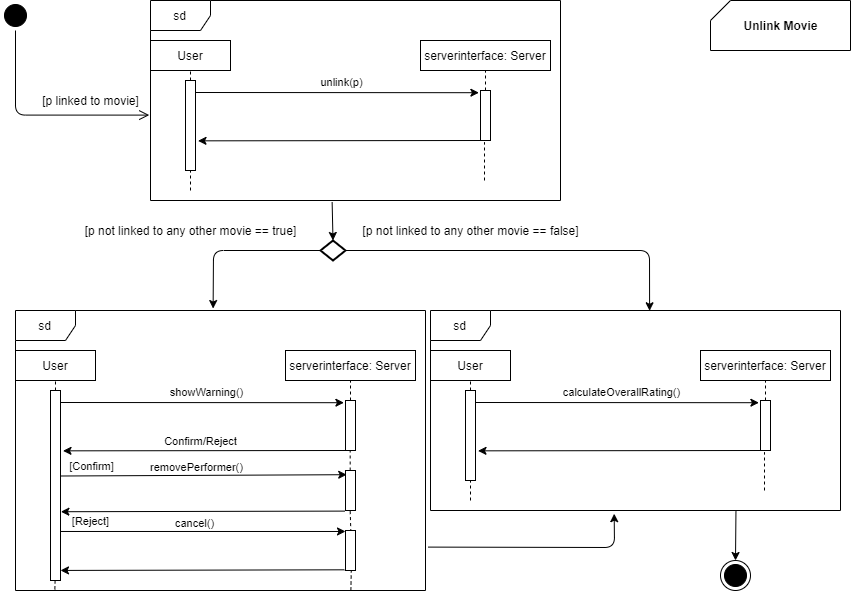
\includegraphics[width=\textwidth]{./images/iod.png}
	\caption{The interaction overview diagram}
	\label{iod}
\end{figure}

\begin{lstlisting}[caption={Contracts written in OCL},label={contracts2}]
	context Movie::unlink(performer)
	pre  self.performers[performer] -> not isEmpty()
	post self.performers[performer] -> isEmpty()
	
	context MovieManager::removePerformer(performer)
	pre forAll(movie | movie.performers[performer] -> isEmpty())
	post self.performers[performer] -> isEmpty()
	
	context Movie::calculateOverallRating()
	post self.overallRating = 0.5 * (self.mean(self.performers.getRatings()) + self.rating)
\end{lstlisting}

\newpage

Based on the IOD and the specified contracts the CTS matrix gets defined and leads to the CTS shown in \autoref{cts}.

\begin{longtable}[h]{llll}
	Operations & Pre & Post & Composite States \\
	$O_{1}$ & $S_{0}$ & $S_{1}$ OR $S_{2}$ & A \\
	$O_{2}$ & $S_{1}$ & $S_{3}$ OR $S_{4}$ & B \\
	$O_{3}$ & $S_{3}$ OR $S_{4}$ & $S_{2}$ & \\
	$O_{3}$ & $S_{2}$ & $S_{5}$ & \\
\end{longtable}

The operations can be thought of as the transitions in the CTS (visualized as arrows), whereas the states match the specified postconditions (maybe thought of as starting points of arrows).

\begin{figure}[h]
	\centering
	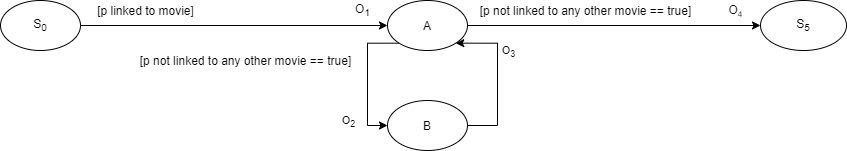
\includegraphics[width=\textwidth]{./images/cts.png}
	\caption{Contracts Transition System}
	\label{cts}
\end{figure}

Based on a coverage criterion the test paths get derived. Different from the first approach no test scenarios get generated. The paper only shows a new more low-level, graphical approach to generate test paths as this was even a suggested improvement from the authors of the first paper. 

\section{Comparison} \label{comparison}

To better compare the two approaches a synthesis matrix based on the following questions is provided:

\begin{enumerate}
	\item Description of the approach (What does the approach do?)
	\begin{enumerate}
		\item Which artifacts and relations between artifacts are used in this approach? Which artifacts are created in the course of the approach? How are the artifacts characterized?
		\item What is required and/or input for the application of the approach?
		\item What steps does the approach consist of? Which information is used in which step and how? What are the results of the individual steps?
	\end{enumerate}
	\item Benefits of the approach (Whom does the approach help and how?)
	\begin{enumerate}
		\item Which usage scenarios are supported by the approach?
		\item Which stakeholders are supported by the usage scenarios?
		\item Which knowledge areas from SWEBOK can be assigned to the usage scenarios?
	\end{enumerate}
	\item Tool support for the approach (What tool support is available?)
	\begin{enumerate}
		\item What tool support is provided for the approach?
		\item Which steps of the approach are automated by a tool? Which steps are supported by a tool, but still have to be executed manually? Which steps are not supported by a tool?
	\end{enumerate}
	\item Quality of the approach (How well does the approach work?)
	\begin{enumerate}
		\item How was the approach evaluated?
		\item What are the (main) results of the evaluation?
	\end{enumerate}
\end{enumerate}

\begin{longtable}[h]{p{0.5cm}p{0.5\textwidth}p{0.5\textwidth}}
	Nr. & Approach \cite{ClementineNebut2006} & Approach \cite{NajlaRaza2007} \\
	1a & 
	Use cases describing the basic operations in the transition system. Contracts that are attached to the use cases describing the states in the transition system. A contract consists of pre- and postconditions that specify the system properties to make a use case applicable and which properties are acquired by the system after its application. Parameters to contracts are actors and main concepts of the use case. The transition system (UCTS) itself as a simulation model to derive test objectives. The states in the UCTS are given through the predicates defined in the contracts, the transitions are triggered when applying an instantiated use case. Test objectives describing the test paths. UC-System as a third party tool to build the UCTS and to derive test objectives using coverage criteria. Use case scenarios to build test scenarios from test objectives. Use case scenarios contain the main messages exchanged between the tester and the SUT, they define how the system has to be simulated to perform a use case and how to react to the simulation. UC-SCSystem to generate executable test scenarios.  & 
	IODs holding all scenarios and operations of a use case. Operations can either be interaction uses or sequence diagrams inside the IOD and define the state transitions. Contracts written in OCL that are attached to the operations describing the states in the transition system. The CTS describing the transition system. Test paths derived from the CTS using coverage criteria.  \\
	1b & 
	Use cases, contracts written as logical expressions, use case scenarios (sequence diagrams), initial system state, selected coverage criterion, and additional use case scenario parameters. & 
	IODs, contracts written in OCL, selected coverage criterion, possibly manual resolving of conflicts in the CTS matrix. \\
	1c &
	To express the ordering constraints between use cases, each use case is attached by a contract. To simulate the use cases, the set of formal parameters of the contracts are replaced with all possible combinations of their actual values. The use cases are then called \textit{instantiated}. To apply an instantiated use case the precondition of its contract must match with the current simulation state. Afterwards the simulation state is updated according to the postcondition of the use case. Exhaustively simulating the system results in the UCTS. To derive test objectives the transition system is traversed according to one of the predefined coverage criteria AE, AV, AIUC, AV-AIUC, or APT. To build test scenarios a use case scenario can replace a use case at a certain stage of execution if the state reached at this stage locally implies the precondition of the use case scenario. Executable test scenarios are generated by the prototype-tool UC-SCSystem. &
	Each operation in the IOD was enriched with its own contract written in OCL. To build the CTS, first all operations have to be identified from the IOD. The operations are taken from the sequence diagrams or from other operations expressed as interaction occurrences in the IOD. Using the contracts of operations, the states for the CTS are identified. Eventually, conflicts in the CTS have to be resolved such as logical if-then-else conditions, equal contract statements, or join nodes. After the CTS was built, test paths are derived from the CTS by applying a coverage criterion, which is either state-, transition- or transition pair coverage. \\
	2a & 
	Automatic test generation from use cases and use case scenarios. Requirement validation by identifying inconsistencies, underspecifications, and invariants. & 
	Deriving test paths from IODs. Further requirement validation on use case level.\\
	2b & 
	Test writers / Developers, Requirement Engineers. &
	Test writers / Developers, Requirement Engineers. \\
	2c &
	Software Requirements (definition of a software requirement, functional requirements, acceptance tests), Software Testing (model-based techniques, objectives of testing, evaluation of the tests performed), Software Engineering Models and Methods (preconditions, postconditions and invariants, behavioral modeling, analysis for consistency, and correctness, traceability). &
	Software Requirements (definition of a software requirement, functional requirements, acceptance tests), Software Testing (model-based techniques), Software Engineering Models and Methods (preconditions, postconditions and invariants, behavioral modeling, analysis for consistency and correctness). \\
	3a & 
	Dedicated editor to design use cases with contracts, UC-System to build the UCTS simulation model, and to derive test objectives from it. UC-SCSystem to exchange the use cases by use case scenarios in order to build the executable test case scenarios. & 
	UML 2.0 as a standard for IODs, OCL as a formal language to write the contracts, prototype tool to derive test paths. \\
	3b & 
	Writing the use cases and contracts is supported by a dedicated editor, but has to be done manually. Deriving test objectives from use cases and contracts through the transition system is done automatically by UC-System. Use case scenarios have to be specified manually, the generation of test scenarios works semi-automatically with UC-SCSystem as it may need additional parameters from the tester. & 
	Only the IOD and contract specification has to be done manually, the complete approach was then automized by a prototype tool. \\
	4a & 
	The approach was evaluated by looking at the statement coverage of three sample programs and the efficiency of test case scenario generation. & 
	The approach was evaluated by looking at the number of test paths generated to cover all success scenarios and fault detections. \\
	4b &
	Code coverage with the most coverage criteria was around 80\%. The coverage criteria differ in efficiency. AE, AV, and AV-AIUC perform with low efficiency, the sets of test cases are larger than in AIUC and APT. APT reaches 100\% functional test coverage with only 15 test case scenarios. Testing robustness leads to a high number of generated test case scenarios that only cover about 50\% of the corresponding code. The approach is good for functional testing, but bad for robustness testing. &
	Using the transition criterion to derive test paths leads to a reasonable amount of test paths and covers all alternative flows in the IOD, but is not suitable for fault detection at any time. The transition pair coverage criterion guarantees the maximum fault detection, but leads to a high amount of test paths. State coverage captures all success scenarios. \\
\end{longtable}

Both approaches have a transition system as a core component in common. Both use contracts to define the states in the transition system. A transition can be applied in case the precondition is fulfilled, the state is then updated according to the postcondition. The transition system is used to derive test paths. Furthermore, both approaches define coverage criteria to generate a certain amount of test cases from the transition system. Both have the AE/transition coverage criterion and AV/state coverage criterion in common. Using this core idea it is also easy in both approaches for requirement engineers to validate their specified requirements during the simulation of the transition system. Both papers draw a similar conclusion, that the core approach is helpful to generate functional test case scenarios for the requirements, nevertheless, there is a lack to achieve a comparable coverage for robustness code for fault detection.

Nevertheless, the two approaches differ in their case of application. While \cite{ClementineNebut2006} uses use cases to automatically generate system-level tests, \cite{NajlaRaza2007} restricts to generate test paths for a specific use case. It therefore does not need additional use case scenarios as an input like \cite{ClementineNebut2006} to generate test scenarios as these are already natively given in the IOD. 

Besides the case of application, the input parameters in both approaches are different as well. \cite{ClementineNebut2006} uses requirement-level first-order logical expressions to describe use cases and their contracts. A more graphical approach was chosen in \cite{NajlaRaza2007} by specifying a use case with an IOD instead of using a formal language. 

\cite{ClementineNebut2006} has the special characteristic that it demonstrates an almost fully automized end-to-end test scenario generation process until concrete test execution, which is missing in \cite{NajlaRaza2007}. Nevertheless, this could easily be implemented in \cite{NajlaRaza2007} as well using similar tool support as in \cite{ClementineNebut2006}. 

\section{Conclusion} \label{conclusion}

Both approaches deliver a method on how to bring requirement specification and system test generation closer together, eliminating traceability problems between what was specified and what was implemented. Requirements can easily be validated on their consistency, correctness, and on possible underspecification while at the same time test paths can be derived through traversing a transition system. 

In literature search, a second paper was found that follows the process of automatically generating test paths through traversing a transition system, but this time uses the in \cite{ClementineNebut2006} proposed extension of IODs as a form of activity diagrams instead of use cases as its input besides contracts. To find this article both snowballing and search-term-based techniques were used, whereas the choice of relevant articles was based on previously specified relevance criteria. Eight resulting papers were found according to these criteria, \cite{NajlaRaza2007} was finally chosen. 

Approach \cite{ClementineNebut2006} almost shows a fully automated way to derive executable test scenarios as JUnit tests. Contract enriched use cases using a formal language based on requirement-level first-order logical expressions are used as an input to the simulation model. Through exhaustive simulation, a transition system is build from which test objectives are derived using coverage criteria. It was empirically proven that the AIUC and APT criterion perform the most efficient and the most extensive measured by statement coverage. Giving contract enriched use case scenarios as a second input helps to generate concrete executable test scenarios. 

\cite{NajlaRaza2007} switches from system level to use case level test generation. It uses contract enriched IODs as graphical input and builds a transition system on it. Test paths are generated using the transition coverage criterion. No further methodology was introduced to generate executable test cases, but as the approach is already specified on use case level, the generation of test code is self-explanatory (a similar tool like UC-SCSystem from \cite{ClementineNebut2006} can be used).

One weakness of both approaches remains the capability to generate a sufficient amount of robustness tests for fault detection. Both approaches only rely on contract violations and do not sufficiently cover data variations as test path generation is only based on one initial state chosen by the test creator. Still, for the automatic generation of functional test scenarios, both approaches show industry-standard and highly applicable solutions.
\chapter{Conclusion}
Fusce vitae quam eu lacus pulvinar vulputate. Suspendisse potenti. Aliquam imperdiet ornare nibh. Cras molestie tortor non erat. Donec dapibus diam sed mauris laoreet volutpat. Sed at ante id nibh consectetuer convallis. Suspendisse diam tortor, lobortis eget, porttitor sed, molestie sed, nisl. Integer enim nisl, lacinia in, pretium eu, viverra a, odio. Quisque at quam eget risus placerat porttitor. Suspendisse convallis, elit vitae mattis pharetra, orci nisl ultrices sapien, ac interdum metus lorem iaculis diam. Nunc id nunc sit amet nisl tincidunt congue. Curabitur et sapien.
\chapter{Glossary} \label{glossary}

\textbf{Contract.} A requirement-level logical expression used to express preconditions and postconditions of an \textit{operation}.

\textbf{Coverage criterion.} A criterion used to limit the amount of \textit{test objectives} to be generated. Specifies which paths to traverse in the context of the traversal of a \textit{transition system}. 

\textbf{Interaction Overview Diagram (IOD).} A special form of activity diagram used to show control flow. Each node in the IOD represents either an interaction diagram (sequence diagrams) or interaction occurrences that show an \textit{operation} invocation.

\textbf{Object Constraint Language (OCL).} A declarative language in the UML standard used to define \textit{contracts}. 

\textbf{Operation.} An abstract term used to describe a state transition in a \textit{transition system}. Is equal to a \textit{use case} in \cite{ClementineNebut2006} or to an interaction diagram/interaction occurrence in \cite{NajlaRaza2007}.

\textbf{Test case.} Tests a single \textit{use case}.

\textbf{Test objective.} A synonym for test path as a combination of abstract \textit{operations} to be composed into one \textit{test scenario}. 

\textbf{Test scenario.} A sequential composition of \textit{test cases}.

\textbf{Transition system.} Used to derive \textit{test scenarios} by helping to generate \textit{test objectives} through its traversal. Consists of states and transitions, where states are given by \textit{contracts} and transitions are given by \textit{operations}. 

\textbf{UC-System.} A prototype/interpreter-tool used to build a \textit{transition system} in \cite{ClementineNebut2006} and to derive \textit{test objectives} from it. 

\textbf{UC-SCSystem.} A prototype-tool using \textit{use case scenarios} to derive executable \textit{test scenarios} as JUnit tests in \cite{ClementineNebut2006}. 

\textbf{Use case.} An abstract, requirement-level term used to describe a main functionality of a system.

\textbf{Use case scenario.} A synonym for sequence diagram in case of \cite{ClementineNebut2006}.

\textbf{XML Metadata Interchange (XMI).} XML based metadata interchange format gained from an \textit{Interaction Overview Diagram} in \cite{NajlaRaza2007} to generate a \textit{transition system}.


%% Bibliography
\bibliographystyle{plainnat}
%\bibliography{literature.bib}%Bibliography file name

\begin{thebibliography}{9}

\bibitem{KunChen2005} Chen, K, Zhang, W., Zhao, H.: An approach to constructing feature models based on requirements clustering.
In: 13th IEEE International Conference on Requirements Engineering (RE05). pp. 31-40. (2005)

\bibitem{RichtigesZitierenTUDresden} Institut für Geographie   
Lehrstuhl für Allgemeine Wirtschafts- und Sozialgeographie: An Hinweise zum wissenschaftlichen Arbeiten.
\url{http://www.geogr.uni-jena.de/fileadmin/Geoinformatik/Lehre/backup_05_2007/pdf-dokumente/Skript_WissArbeiten.pdf}

\bibitem{ClementineNebut2006} Nebut, C., Fleurey, F., Le Traon, Y., Jézéquel, J.-M.: Automatic Test Generation: A Use Case Driven Approach.
In: IEEE Transactions on Software Engineering (Volume: 32, Issue: 3, March 2006).
https://doi.org/10.1109/TSE.2006.22.

\bibitem{NajlaRaza2007} Raza, N., Nadeem, A., Iqbal, M. Z. Z.: An Automated Approach to System Testing based on Scenarios and Operations Contracts.
In: Seventh International Conference on Quality Software (QSIC 2007).
https://doi.org/10.1109/QSIC.2007.4385504.

\bibitem{FelixHausberger2020} Hausberger, F.: Research planning, research and mid-term presentation, \url{https://github.com/fidsusj/SWE-Seminar}, last accessed 2021/01/10.

\bibitem{MonalisaSarma2007} Sarma, M., Mall, R.: System Testing using UML Models.
In: 16th IEEE Asian Test Symposium (ATS 2007).
https://doi.org/10.1109/ATS.2007.102.

\bibitem{RosziatiIbrahim2007} Ibrahim, R., Saringat, M. Z., Ibrahim, N., Ismail, N.: An Automatic Tool for Generating Test Cases from the System's Requirements.
In: 7th IEEE International Conference on Computer and Information Technology (CIT 2007).
https://doi.org/10.1109/CIT.2007.116.

\bibitem{LizheChen2010} Chen, L., Li, Q.: Automated test case generation from use case: A model based approach.
In: 2010 3rd International Conference on Computer Science and Information Technology.
https://doi.org/10.1109/ICCSIT.2010.5563772.

\bibitem{XiaojingZhang2015} Zhang, X., Tanno, H.: Requirements document based test scenario generation for web application scenario testing.
In: 2015 IEEE Eighth International Conference on Software Testing, Verification and Validation Workshops (ICSTW).
https://doi.org/10.1109/ICSTW.2015.7107465.

\bibitem{LipingLi2008} Li, L., Miao, H.: An Approach to Modeling and Testing Web Applications Based on Use Cases.
In: 2008 International Symposium on Information Science and Engineering.
https://doi.org/10.1109/ISISE.2008.265.

\bibitem{YGKim1999} Kim, Y. G., Hong, H. S., Cho, S. M., Bae, D. H., Cha, S. D.: Test cases generation from UML state diagrams.
In: IEEE Proceedings - Software, Vol. 146, No. 4, pp. 187-192, Aug. 1999.
https://doi.org/10.1049/ip-sen:19990602.

\bibitem{ClementineNebut2003} Nebut, C., Fleurey, F., Le Traon, Y., Jézéquel, J.-M.: Requirements by Contracts allow Automated System Testing.
In: Proceedings of the 14th International Symposium on Software Reliability Engineering (ISSRE November 2003).
https://dl.acm.org/doi/10.5555/951952.952350.

\end{thebibliography}

\listoffigures

\listoftables

\end{document}          
